%PART_1_CHAP_3
\myChapter{A}{spects motivationnels}
%WAIT a Review ok
\begin{resumChap}
Le système éducatif français est donc un écosystème à part entière avec ses propres contraintes et ses propres besoins ainsi que différents acteurs qui le compose.\par%
Motiver ces acteurs à réaliser les tâches qui sont les leurs est un objectif souvent associé à la conception des outils qui leur sont dédiés.
\\\strut\hfill Mais, qu'est-ce qu'être motivé?\hfill\strut\par%
Nous verrons dans ce chapitre comment se définit la motivation et quels sont les modèles théoriques qui lui sont associés, comme la théorie de l'auto-détermination, ou le modèle de Viau.\par%
Plus particulièrement, nous verrons comment la motivation est abordée suivant deux points de vue: \Li celui des prescripteurs (l'Éducation Nationale), \ii celui du monde scientifique.\par%
Nous citerons quelques éléments notoires qui peuvent en être extraits et pouvant être utiles aux pédagogues dans la réalisation de leur travail.\par%
Nous verrons également comment les sciences cognitives sont venues compléter les connaissances sur ces notions au travers de l'analyse des fonctions cognitives et la théorie de la charge cognitive.
\end{resumChap}
\section{La motivation scolaire}\label{sec:motiv}
    Kim \& al~\citeB{kim2015robotics} décrivent la robotique comme un outil d’apprentissage motivant en raison de l’encouragement à l'expérience qui est généré. La motivation est la base de l’engagement~\citeB{green2012academic}, ainsi, la robotique peut être utilisée comme un outil pour engager des enseignants et des élèves dans l'apprentissage des sciences, technologies, ingénieries et mathématiques.
    \subsection{La motivation}
        %\subsection{La motivation}
            %\subparagraph{En général}
                D'un point de vue général, nous pouvons prendre une première définition qui est celle offerte par l'encyclopédie Universalis:
                \citeAtion{motivation}\par%
                Le \sht{cnrtl}, lui, distingue plusieurs définitions suivant le domaine où il est employé. Notamment il distingue un domaine psychopédagogique:
                \citeAtion{motivationCnrtl}\par%
                Nous voyons dans cette seconde définition que la motivation scolaire est restreinte à la seule motivation à apprendre. Mais surtout, ici la motivation est définie comme un ensemble de facteurs dynamiques et non un processus psychologique. Dès lors la motivation est plus facilement catégorisable et mesurable. 
                Il existe certainement autant de définitions de la motivation qu'il existe de modèles cherchants à l'interpréter.
                Une vision courante est celle fournie par la \sht{SDT}~\citeB{black2000effects} qui fait notamment la distinction entre 2 différents types de motivation et leurs conséquences.
            \subparagraph{Intrinsèque}
                La motivation intrinsèque a été étudiée depuis le début des années 1970. La motivation intrinsèque est considérée comme le désir de chercher de nouvelles choses et de nouveaux défis, d’analyser ses capacités, d’observer et d’atteindre un objectif comme par exemple arrêter de fumer. Deci~\citeB{deci1971effects} a montré que certaines activités fournissent leurs propres récompenses inhérentes, et que par conséquent elles ne dépendent pas d'une récompense externe. La motivation vient alors d'un intérêt ou d'un plaisir pour la tâche elle-même et ses finalités. 
                La théorie de l'évaluation cognitive (Cognitive evaluation theory~\citeB{deci2010intrinsic}) est une sous-théorie de la \sht{SDT} qui spécifie les facteurs expliquant la motivation intrinsèque. Elle se concentre sur les besoins de compétence et d’autonomie définis par la \sht{SDT}~\citeS{sec:SDT}. Par ce prisme plusieurs effets ont été mis en lumière~\citeS{sec:illus}, par exemple, Deci a constaté que les réactions positives amélioraient les motivations intrinsèques et que les réactions négatives les diminuaient; Vallerand et Reid~\citeB{vallerand1984causal} sont allés plus loin et ont constaté que ces effets étaient médiés par le contrôle perçu. L'autonomie, cependant, doit accompagner la compétence pour que les gens voient leur comportement comme déterminé par leur motivation intrinsèque. Une autre hypothèse est que la motivation intrinsèque s'épanouit si elle est liée à un sentiment de sécurité et de parenté. Grolnick et Ryan~\citeB{grolnick1989parent} ont trouvé une motivation intrinsèque plus faible chez les enfants qui pensaient que leurs enseignants étaient indifférents ou froids et ne répondaient donc pas à leurs besoins en matière de parenté.
            \subparagraph{Extrinsèque}
                La motivation extrinsèque provient de sources externes. Deci et Ryan ont développé la théorie de l'intégration organismique (organismic integration theory~\citeB{deci2010intrinsic}), en tant que sous-théorie du \sht{SDT}, pour expliquer les différentes manières de réguler les comportements à motivation extrinsèque. Elle détaille les différentes formes de motivation extrinsèque et les contextes dans lesquels elles se développent.
                Cette théorie définit 4 types de motivations extrinsèques définies par leur \cro{lieu} de régulation: 
                \begin{enumerate}\myItemStyle
                    \item Un comportement régulé de l'extérieur: il est exécuté en raison d'une demande externe ou d'une éventuelle récompense. On peut considérer que ces actions ont un lieu de causalité perçu de manière externe~\citeB{decharms1968measuring}, c'est le moins autonome.
                    \item Un comportement régulé par intrusion: c'est le fait de respecter des règles \cro{personnelles} mais qui ne sont pas entièrement acceptées comme des règles émanant directement de l'individu. Deci et Ryan~\citeB{deci1995human} affirment qu'un tel comportement représente normalement une régulation par une estime de soi contingente, citant l'implication de l'ego comme une forme classique d'introjection~\citeB{ryan2000self}. Bien que ce comportement soit impulsé de manière interne, le comportement a un lieu de causalité perçu comme externe. %Puisque la causalité du comportement est perçue comme externe, le comportement est considéré comme non autodéterminé.
                    \item Un comportement régulé par identification: c'est le type de motivation extrinsèque plus autonome que les précédentes. Elle implique de valoriser consciemment un objectif et que les actions exécutées soient considérées comme personnellement importantes. 
                    \item Une régulation intégrée: c'est le type le plus autonome de motivation extrinsèque. Les règles sont totalement assimilées par l'individu: elles sont incluses dans son auto-évaluation et ses croyances sur ses besoins personnels, on dit qu'elles sont internalisées. Elle se rapproche donc fortement de la motivation intrinsèque, mais, comme les objectifs recherchés sont pour des raisons externes à soi-même et non pour le plaisir ou l'intérêt inhérent à la tâche, on continue de parler de motivation extrinsèque. Ryan, Stiller et Lynch~\citeB{ryan1994representations} proposent que l'internalisation ait plus de chance de se produire lorsqu'il existe un sentiment de parenté. Ils ont constaté que les enfants intériorisent les règles extrinsèques de l'école lorsqu'ils se sentent en sécurité et pris en charge par leurs parents et leurs enseignants. L'internalisation de la motivation extrinsèque semble également liée à la compétence dans les activités qui devraient faciliter l'internalisation de ces actions~\citeB{vallerand1997toward}. L'autonomie semble également importante en matière d'internalisation. Ainsi, selon la \sht{SDT}, si un contexte externe permet à une personne d’intégrer la règle, elle doit se sentir compétente, liée et autonome. L'individu doit également comprendre la règle en fonction de ses autres objectifs, afin de favoriser un sentiment d'autonomie~\citeB{kuhl1998decomposing, deci1994facilitating}. %Cela a été soutenu par Deci, Eghrari, Patrick et Leone~\citeB{deci1994facilitating}, qui ont découvert en laboratoire si une personne recevait une raison valable pour un comportement inintéressant, tout en renforçant son sentiment d'autonomie et de parenté, l'intériorisant et en intégrant son comportement.
                \end{enumerate}
        \subsection{Restreint au cadre scolaire}
            Les pouvoirs publics ont une notion relative de la motivation scolaire: il appartient aux enseignants de motiver leurs élèves en leur proposant une pédagogie et un contenu adaptés à leurs profils dans l'objectif du développement des compétences et connaissances prescrites dans les programmes. C'est donc du point de vue de la réussite \tiret{ou de l'échec} qu'est abordée la motivation, ou plutôt, le besoin de re-motivation, de raccrochage.
            \paragraph{Décrochage scolaire}
                On parle de décrochage scolaire lorsqu’un élève quitte l’institution scolaire et arrête son cursus en cours. Plus précisément, selon le code de l'éducation, être décrocheur, c'est \gui{ne pas avoir terminé avec succès le cycle de formation de second cycle du second degré dans lequel le jeune s'était engagé}. Ainsi, est considéré comme décrocheur un élève titulaire d'un CAP, qui poursuit ses études pour le compléter par un second CAP ou pour obtenir un baccalauréat professionnel mais qui arrête sa scolarité sans avoir atteint son objectif. Autrement dit, on peut être décrocheur et diplômé~\citeURL{BO-def} contrairement aux élèves dits en échec scolaire.
            \paragraph{L'échec scolaire} 
                Il correspond au fait qu'un élève sorte de formation initiale sans l'obtention d'un diplôme d'État (BAC, CAP, \etc). En 2010, ils étaient 140 000 et ce chiffre est actuellement décroissant: 110 mille en 2014 et 107 en 2015. Bien évidemment, un bon moyen de lutter contre ce phénomène est de ne pas avoir de décrocheur et de favoriser la réussite \cro{normale}.
            \paragraph{Réussite éducative}
                Le pacte pour la réussite éducative, publié le 7~novembre 2013, définit la réussite éducative comme la recherche du développement harmonieux de l'enfant et du jeune. Ce pacte cherche \gui{à favoriser la réussite des élèves et leur bien-être en développant la cohérence et la complémentarité des actions dans l'école et hors de l'école et en transformant les pratiques pédagogiques et éducatives à l'échelle des territoires, plusieurs actions sont menées dans ce sens~\citeURL{BO-reusiste-sco}}. Notamment nous pouvons citer l'innovation comme étant un des axes choisi par le système éducatif pour maximiser cette réussite, et plus particulièrement souligner le rôle du \sht{Cnire} qui a pour principal objectif de promouvoir l'esprit d'innovation en matière de réussite scolaire et de réussite éducative: elle propose 3 pistes de travail: \Li l'ouverture de l'école (notamment aux parents), \ii le développement des compétences et \iii l'amélioration de l'engagement (des élèves et des personnels).
    \subsection{L'engagement}
        En psychologie sociale le terme d'engagement fait référence à la vision théorisée par Kiesler et Sakumura~\citeB{kiesler1971psychology}. Il a été développé et raffiné par de nombreux auteurs comme Stanley Milgram ou Jean-Léon Beauvois. La théorie de l'engagement englobe un nombre conséquent de techniques et procédures. Régulièrement utilisés via des stratégies de manipulation en marketing, ces concepts font souvent l’œuvre d'utilisation malhonnête. Prendre connaissance de leur existence permet de s'en protéger.
        Ici, l'engagement sera abordé dans sa vision 'informatique', c'est à dire comme \gui{une mesure de la popularité\footnote{Le fait d'être connu et aimé d'un groupe d'individus, les sentiments favorables qu'ils portent envers une personnalité ou une chose}}: l'engagement est défini comme le ratio du nombre d'utilisateurs quotidiens d'une application sur le nombre d'utilisateurs mensuels de l'application (source wikipédia~\citeURL{engagement}).\par%
        Plus particulièrement, nous définirons cet engagement en fonction de sa persistance dans le temps. Ainsi, nous parlerons d'une part de l'engagement à court terme et d'autre par d'engagement à long terme.
        %\paragraph{À court terme}%\paragraph{À long terme}
        Pour le premier, nous y ferons référence pour caractériser l'engagement dans une activité donnée, correspondant à un atelier scolaire classique de 2 à 4h. Par extension, le ré-engagement concernera la mesure de la \cro{popularité} lors de l'intégration d'une seconde activité. De là, nous définissons la seconde: l'engagement à long terme est vu comme une suite de ré-engagement à court terme. Et ainsi, la persévérance est la capacité à rester engagé ou se re-engager dans une activité sur laquelle l'individu décroche.\par%  
        Du point de vue de la robotique, l’article de Kim, C \& al~\citeB{kim2015robotics} précise que l’engagement cognitif (au sens de focus attentionnel et de mobilisation de ressources) est plus fréquent dans les petits groupes collaboratifs, et que le fait d’essayer, de questionner, d’échanger des idées ou des explications au sein du groupe renforcerait cet engagement. De plus, le fait de prendre des initiatives serait un indicateur d’un haut niveau d’engagement comportemental.
\section{Modèle théorique de la motivation}
    \subsection{La théorie de l'autodétermination}\label{sec:SDT}
        Aussi appelée \glsdesc{SDT}, est une macro théorie de la motivation.
        Il concerne la motivation derrière les choix faits par les individus sans influence extérieure. La \sht{SDT} cherche à déterminer dans quelle mesure le comportement d'un individu est motivé et auto-déterminé. \citeB{ryan2000self,deci2012motivation,ryan2017self}
        Dans les années 1970, la recherche sur la \sht{SDT} découlait d'études comparant les motifs intrinsèques et extrinsèques, et d'une compréhension croissante du rôle de la motivation intrinsèque dans le comportement d'un individu~\citeB{lepper1973undermining}. Ce n'est qu'au milieu des années 1980 que la \sht{SDT} a été officiellement introduite et adoptée: acceptée comme une théorie empirique solide. Les recherches sur l'application du \sht{SDT} à différents domaines de la psychologie sociale ont considérablement augmenté depuis les années 2000. 
        Edward L. Deci et Richard Ryan ont ensuite développé les travaux initiaux faisant la distinction entre motivation intrinsèque et motivation extrinsèque et proposé trois principaux besoins intrinsèques liés à l'autodétermination.\citeB{deci1991motivation,kernis1995efficacy} Selon Deci et Ryan, les trois besoins psychologiques incitent le \textit{self} à adopter un comportement et à spécifier les nutriments essentiels à la santé psychologique et au bien-être d'un individu. Ces besoins sont dits universels, innés et psychologiques et incluent le besoin de compétences, d'autonomie et de relations~\citeB{chirkov2003differentiating}.
        \paragraph{Autonomie}\nocite{decharms1968measuring}
            Deci a constaté que le fait d'offrir aux gens des récompenses extrinsèques pour un comportement intrinsèquement motivé minait la motivation intrinsèque, car ils s'y intéressaient moins. Les comportements initialement motivés intrinsèquement deviennent contrôlés par des récompenses externes, ce qui sape leur autonomie~\citeF{fig:motiv1}.
            Des recherches ultérieures menées par Amabile, DeJong et Lepper~\citeB{amabile1976effects} ont montré que d'autres facteurs externes tels que les délais, qui limitent et contrôlent, diminuent également la motivation intrinsèque.
            Les situations qui donnent de l’autonomie plutôt que de la retirer ont également un lien similaire avec la motivation. Des études portant sur le choix ont montré que le fait d'augmenter le nombre d'options et de choix d'un participant augmente sa motivation intrinsèque~\citeB{zuckerman1978importance}.
        \paragraph{Relations}
            Le fait de vouloir développer et entretenir des relations sociales est un phénomène inné à notre espèce grégaire. Ainsi des hypothèses telles que la volonté d'appartenance~\citeB{baumeister1995need} ou d'attachement~\citeB{frodi1985correlates} de l'individu à un groupe ou une catégorie sociale, semblent être de bonnes hypothèses pour constituer les déterminants motivant l'individu dans l'exécution de son comportement. Le critère de stabilité de l'individu dans ce groupe et la sécurité (psychologique) qu'elle implique semble également de bon indicateur pour prédire l'engagement d'un individu dans une activité donnée.
        \paragraph{Compétences}
            Deci, et d'autres~\citeB{harter1978effectance,white1963ego}, ont constaté que le fait de donner aux personnes un retour positif inattendu sur une tâche accroît la motivation intrinsèque des gens à le faire, ce qui signifie que ce retour était dû au fait que le retour positif répondait au besoin de compétence des personnes. En fait, donner une rétroaction positive sur une tâche ne servait qu'à accroître la motivation intrinsèque des personnes et à diminuer la motivation extrinsèque pour la tâche.
            Vallerand et Reid~\citeB{vallerand1984causal} ont constaté que la rétroaction négative avait l'effet inverse c'est à dire qu'elle diminue la motivation intrinsèque en supprimant le besoin de compétence des personnes.
    \subsection{La théorie du besoin d’accomplissement}\label{sec:accomplissement}
        Cette théorie présente le besoin d'accomplissement de soi comme une finalité ultime à toute source de motivation; constamment elle dirige notre action. Ainsi, placées devant une tâche nos croyances préalables vont nous permettre de déterminer un résultat probable quantifiable: ayant une valeur et générant une attente~\citeB{atkinson1957motivational, elliot20012}. Dès lors, l'individu va choisir de s'engager, ou non, dans une action et régulera ses efforts en fonction du résultat attendu; une performance pourra alors être mesurée.\par%
        \begin{figure}[!h]
            \centering
            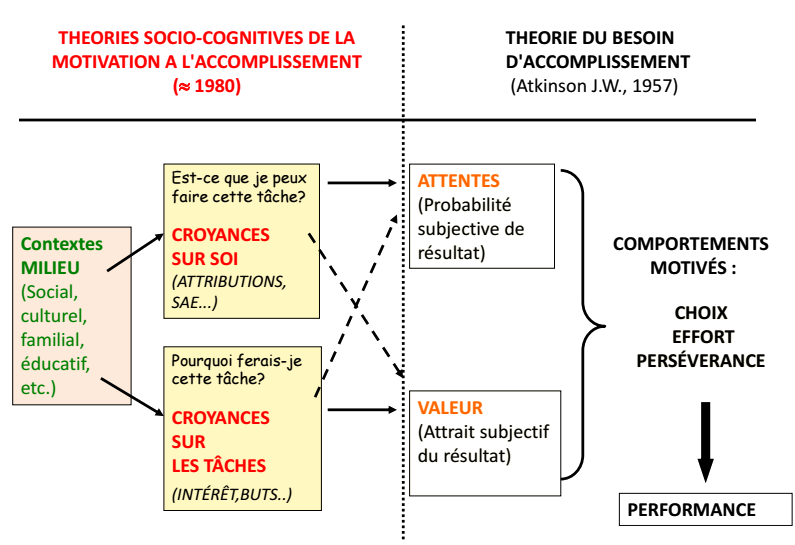
\includegraphics[width=0.8\linewidth]{Figures/Atkinson-besoin_accomplissement.png}
            \caption{Théorie du besoin d’accomplissement, Atkinson~\citeB{atkinson1957motivational}}
            \label{fig:atkinson}
        \end{figure}%\par%
        Contrairement à Maslow~\citeB{mcleod2007maslow}, qui stratifiait différents besoins sous forme de pyramide, Dweck et Elliott \citeB{dweck1986motivational,elliott1988goals} ne définissent qu'un unique besoin et donc un unique but mais qui se décline en plusieurs sous-buts: la maîtrise et la performance.
    %\subsection{La théorie du but d’accomplissement de soi}
        \begin{figure}[!h]
            \centering
            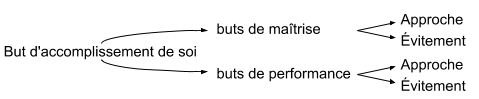
\includegraphics[width=0.9\linewidth]{Figures/Dweck-but_accomplissement.png}
            \caption{Théorie du but d’accomplissement de soi, Dweck et Elliott~\citeB{dweck1986motivational,elliott1988goals}}
            \label{fig:dweck}
        \end{figure}\par%
        \begin{itemize}\myItemStyle
            \item But de maîtrise-approche: \gui{Mon objectif est de maîtriser complètement le contenu présenté dans ce cours}
            \item But de maîtrise-évitement: \gui{Mon objectif est d’éviter de ne pas apprendre moins que ce que je pourrais dans ce cours.}
            \item But de performance-approche: \gui{Mon but dans ce cours est de bien réussir par rapport aux autres étudiant(e)s}
            \item But de performance-évitement: \gui{Mon but est d’éviter de faire moins bien que les autres étudiant(e)s}
        \end{itemize}\par%
        \begin{table}[!h]
        \footnotesize{}
            \centering
            \begin{tabular}{|c|p{0.175\linewidth}|p{0.175\linewidth}||p{0.175\linewidth}|p{0.175\linewidth}|}
            \hline
                 & \multicolumn{2}{c||}{But de Maîtrise} & \multicolumn{2}{c|}{But de Performance}\\ 
                 & d’approche & d’évitement & d’approche & d’évitement \\ \hline
                Le Pourquoi & motif de développement de sa compétence & motif d’évitement de toute erreur, de non maîtrise du cours & motif de valorisation de sa compétence & motif de protection de sa compétence \\ \hline
                Le Pour Quoi & progrès personnels (critères auto-référencés) & Recherche de perfection (critères auto-référencés) & mieux faire que les autres, obtenir des jugements positifs (critères liés à la comparaison sociale) & éviter de montrer ses faiblesses, éviter des jugements négatifs (critères liés à la comparaison sociale) \\ \hline
            \end{tabular}
            \caption{Théorie du but d’accomplissement de soi, Dweck et Elliott~\citeB{dweck1986motivational,elliott1988goals}}
            \label{tab:acc-de-soi}
        \end{table}\par%
        %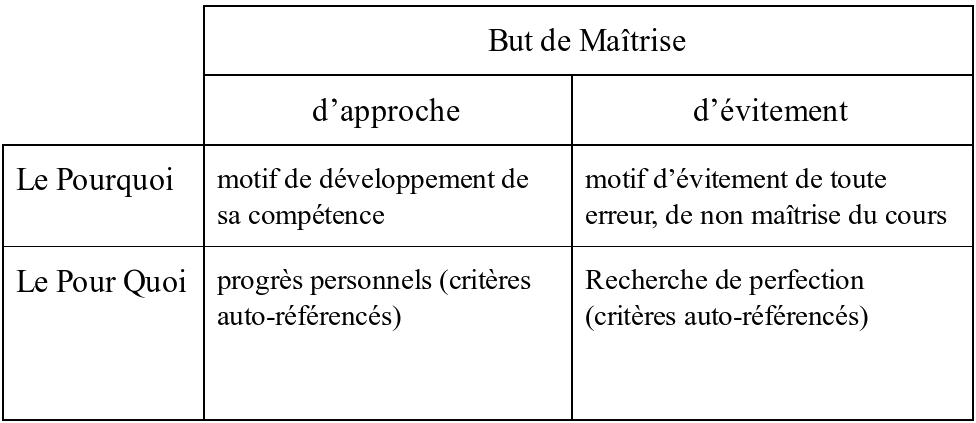
\includegraphics[width=0.48\linewidth]{Figures/Dweck-but_maitrise.png}
        %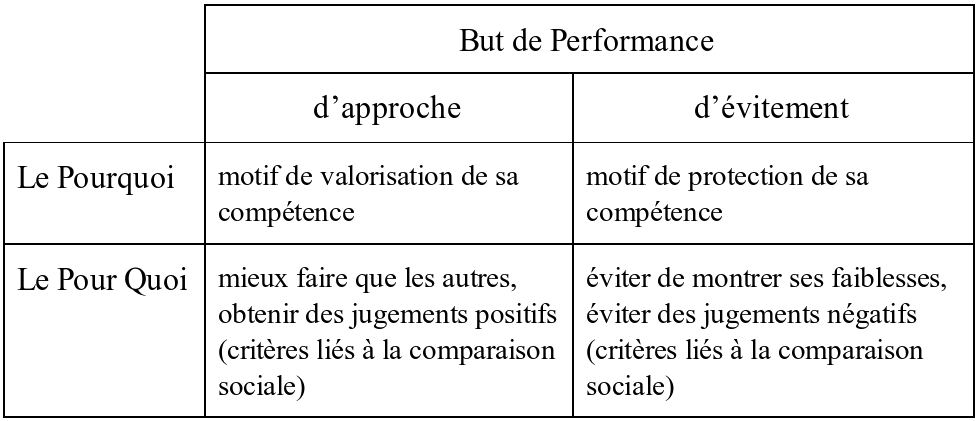
\includegraphics[width=0.48\linewidth]{Figures/Dweck-but_perf.png}
    \subsection{Le modèle de Viau}\label{sec:viau}
        Le modèle de motivation Viau~\citeB{viau1997vers} concerne les éléments qui ont un impact sur la motivation des étudiants.
        Dans son livre \cro{La motivation en contexte scolaire} \citeB{viau1994motivation}, il propose un modèle: selon lui, la motivation des étudiants dépend non seulement du contexte d'apprentissage, mais également de ceux-ci. Le contexte, indépendamment d’eux, peut influencer leur motivation. %Ils comprennent la discipline enseignées, tâches liées à leur apprentissage, mais aussi relations entre étudiants, enseignants, administration, \etc.
        Viau définit sept composantes liées à l'étudiant qu'il divise en deux groupes: les déterminants et les indicateurs. Les déterminants sont liés au contexte de la manière dont l'étudiant appréhende les tâches.
        \begin{figure}[!h]
            \centering
            \label{fig:ViauModel}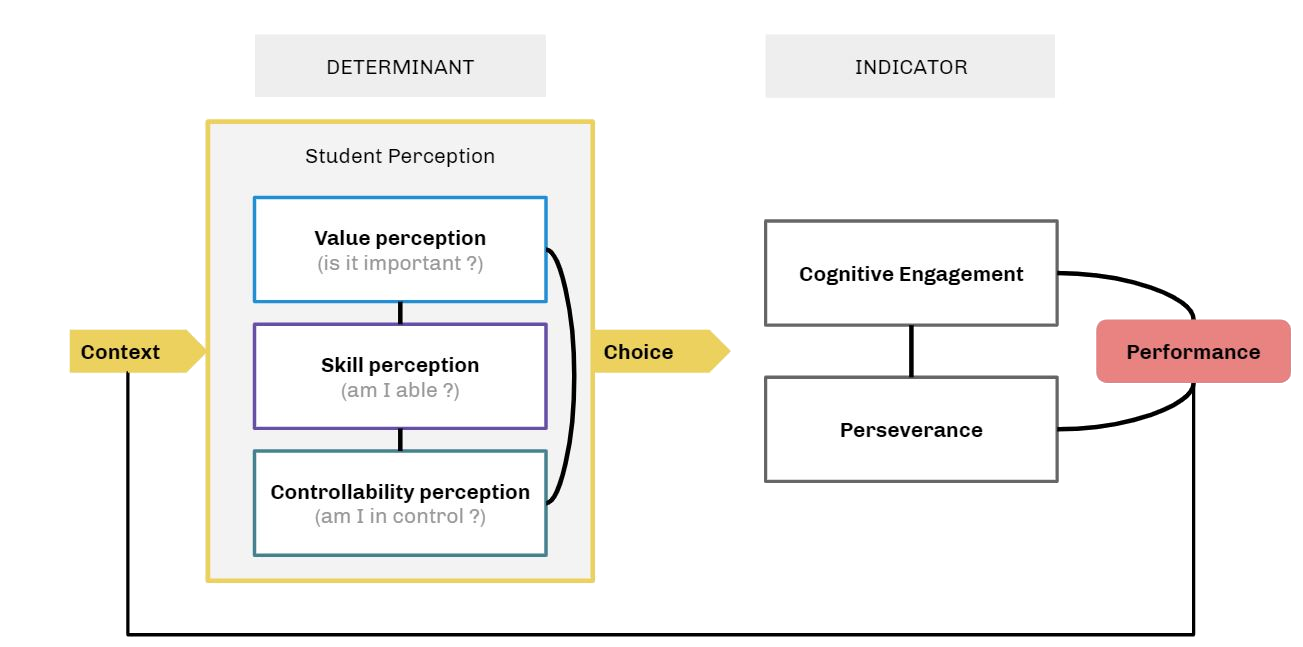
\includegraphics[width=0.9\linewidth]{Figures/ViauModel.png}
            \caption{Modèle de Viau~\citeB{viau1997vers}}
        \end{figure}\par%
        \paragraph{Les déterminants}
            \begin{itemize}\myItemStyle
            \item La perception de la valeur d'une activité: elle correspond au jugement subjectif de l'élève sur l'intérêt d'une activité pour atteindre un objectif. Est-ce pertinent du point de vue de l'étudiant?
            \item La perception de ses propres compétences: c'est l'auto-évaluation de l'élève sur sa capacité à effectuer une activité demandée.
            \item La perception de la contrôlabilité: c'est le niveau de contrôle perçu par l’élève lors de la réalisation d'une activité. Les élèves peuvent-ils influencer l'avancement de l'activité par leurs choix? Cela peut être créé en responsabilisant les étudiants en leur permettant de faire des choix. L'autorité et le monopole du professeur peuvent faire tomber ce sentiment de choix.
            \end{itemize}\par%
        \paragraph{Les indicateurs}
            \begin{itemize}\myItemStyle
            \item \cro{Le choix de réaliser une activité}: un élève peut choisir de réaliser ou non les tâches demandées par l'enseignant, en fonction du degré de motivation.
            \item \cro{Persévérance}: elle est liée au temps que l'étudiant investit dans son apprentissage et aux ressources qu'il y déploie.
            \item \cro{L'engagement cognitif}: On dit que l'étudiant est impliqué cognitivement s'il applique des stratégies d'apprentissage et d'autorégulation dans l'exercice de ses activités.
            \item \cro{Performance des étudiants}: elle est influencée par les trois indicateurs précédents. Ici, il fait référence à l'utilisation par les étudiants de diverses stratégies, connaissances et savoir-faire pour atteindre leurs objectifs.
            \end{itemize}\par%
        Dans ce modèle, les différentes composantes sont interconnectées, ce qui implique que la dynamique de motivation de l'étudiant change progressivement.
\section{D'autres déterminants de la motivation}
    \subsection{Le Flow et la ZPD}
        \strut
        \begin{figure}[!h]
          \begin{minipage}{0.325\linewidth}
              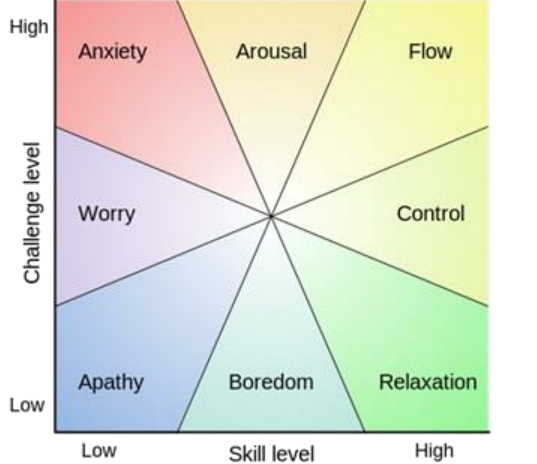
\includegraphics[width=\linewidth]{Figures/Nakamura-FlowModel.png}
              \caption{The FLOW Model, Nakamura~\citeB{nakamura2014concept}}\label{fig:FlowModel}
          \end{minipage}
          \hfill
          \begin{minipage}{0.6\linewidth}
          \myDefautStyle
              La gestion de la difficulté est un point primordial. La progression doit rester croissante tout au long de l'apprentissage mais sans s'écarter de la \glsdesc{ZPD}. C'est également ce que développe Csikszentmihalyi et Nakamura avec \glsdesc{flow} théorie. Ainsi l'activité proposée doit être suffisamment libre pour que l'élève trouve sa propre trajectoire développementale.
          \end{minipage}
        \end{figure}
    \subsection{Le sentiment d’efficacité personnelle}
        Bandura~\citeB{bandura2007auto} définit le \glsdesc{SAE} comme correspondant à l’évaluation subjective de l’apprenant sur ses propres capacités (connaissances et compétences) à accomplir une tâche donnée. Mais aussi sur l'évaluation de ses propres performances à la réalisation de cette tâche. De là, les performances estimées (et réactualisées durant la tâche) déterminent la quantité (temps passé à \dots) et la qualité  (stratégies) de l’effort fourni par l'apprenant.
    \subsection{Les perceptions attributionnelles}
        Pour Weiner~\citeB{weiner1985attributional}, les perceptions attributionnelles lors de la réussite ou de l'échec dans une tâche\citeB{barbeau1991pour}, ont 4 attendus en terme de responsabilité: \Li les aptitudes personnelles (suffisantes ou manquantes), \ii la difficulté de la tâche (suffisante ou trop dure), \iii la quantité d’efforts fournis par l'individu (suffisant ou insuffisant), \iiii la chance. Ces 4 responsabilités sont à moduler selon 3 dimensions causales: la provenance (interne/externe), la stabilité, la contrôlabilité \eg la chance est externe, instable et incontrôlable; les aptitudes personnelles sont internes, stables et contrôlables. Ainsi, un élève peut justifier son échec à un examen par: le manque de chance, une difficulté trop grande, un manque d'aptitudes personnelles ou un effort trop faible suivant ses états mentaux \cro{du moment}.
    \subsection{La contrôlabilité}\label{sec:contro}
        Pour Pintrich~\citeB{pintrich1991manual}, et Murayama 3 concepts sont prédominants:
        \begin{enumerate}\myItemStyle
            \item La planification de l'effort à fournir: \gui{Avant d’étudier en détail une nouvelle partie de cours, je la parcours souvent rapidement pour voir comment elle est organisée} \item L'auto-contrôle durant l'exécution de la tâche: \gui{Je me pose des questions pour m’assurer que je comprends les points étudiés du cours}
            \item La régulation dans la sélection des stratégies mises en œuvre: \gui{Si les chapitres à étudier sont difficiles à comprendre, je change ma façon d’étudier.}
        \end{enumerate}{}\par%
        Permettre à l'apprenant de maîtriser ces dimensions favoriserait ainsi son engagement et sa motivation à réaliser une tâche donnée.
\section{Références illustrées}\label{sec:illus}
    Frédéric Duriez, illustrateur, nous présente sur son blog~\citeURL{motiv_pic} une série de plaquettes vulgarisant l'évolution dans le domaine scientifique sur les questions de la motivation.
    Sa première illustration concerne le psychologue Harry Harlow~\citeB{harlow1950learning} qui en 1949 a constaté que, durant la phase de familiarisation, les macaques s'étaient \cro{pris au jeu} et ont tenté de résoudre les énigmes qui constituent le matériel de sa future expérience, par plaisir; car à ce stade aucune récompense ne leur était fournie pour le travail effectué.\par%
    Ce n'est que vingt ans plus tard que Deci~\citeB{deci1971effects} expérimente une situation similaire avec des humains. Des individus sont invités à résoudre le cube de soma sans promesse de récompense. Si on les rémunère, ils continuent.
    Mais lorsqu'on arrête la rémunération, ou si elle paraît très faible, ils se démotivent et leurs performances baissent par rapport au groupe test qui n'a jamais reçu de récompense.
    À la suite de Deci et Ryan, Daniel Pink~\citeB{pink2011verite} insiste sur la différence entre les motivations extrinsèques et les motivations intrinsèques.
    \begin{figure}[!h]
    \begin{minipage}{0.475\linewidth}
        \centering
        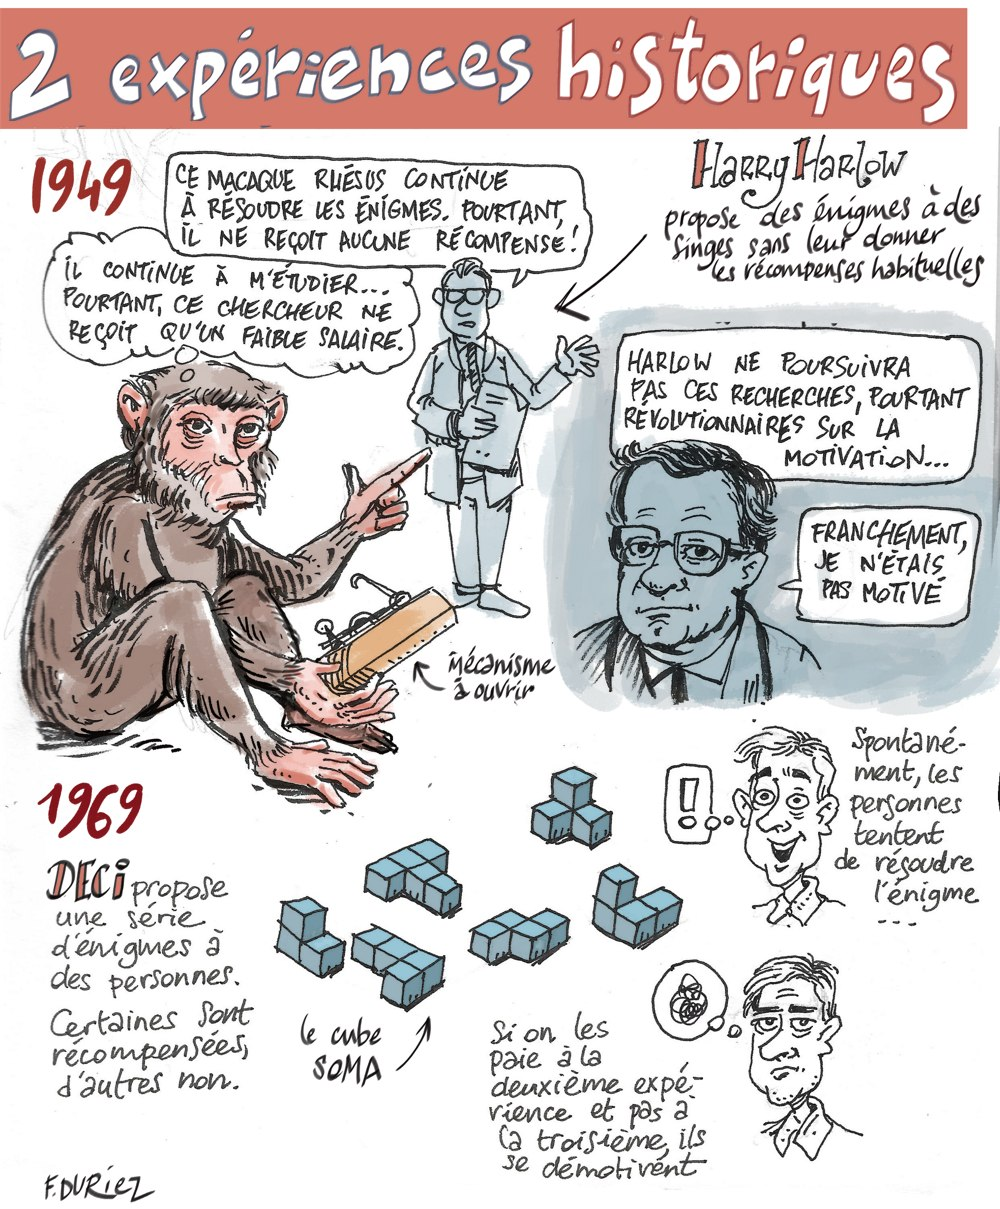
\includegraphics[width=\linewidth]{Figures/Duriez-motiv1.jpg}
        \caption[Harry Harlow~\citeB{harlow1950learning} \& Edward Deci~\citeB{deci1971effects}]{H.~Harlow~\citeB{harlow1950learning} \& E.~Deci~\citeB{deci1971effects}, \textit{ill.} F.~Duriez~\citeURL{motiv_pic}}
        \label{fig:motiv1}
    \end{minipage}
    \hfill
    \begin{minipage}{0.475\linewidth}
        \centering
        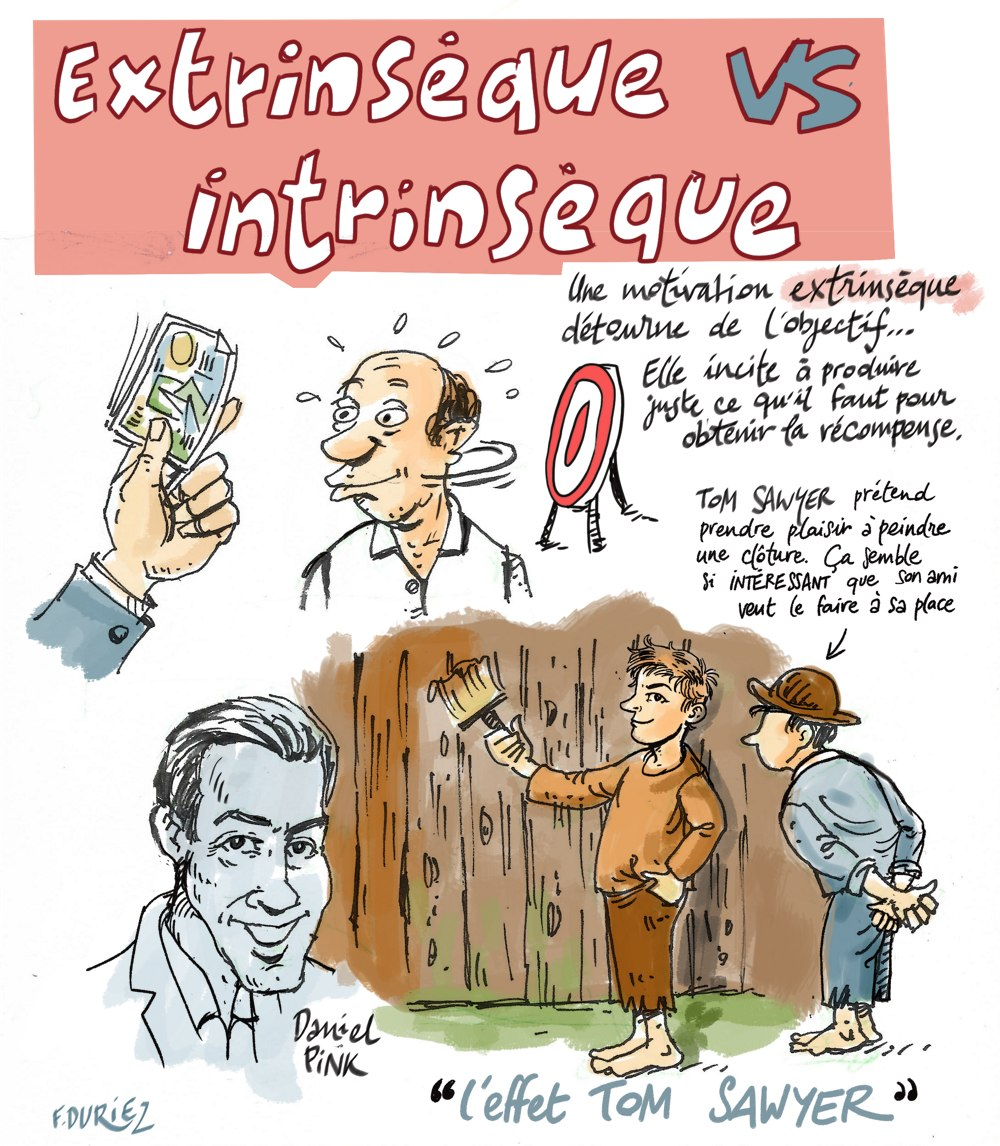
\includegraphics[width=\linewidth]{Figures/Duriez-motiv2.jpg}
        \caption[Effet de la rémunération, Deci~\citeB{deci1971effects} \& effet Tom Sawyer, Pink~\citeB{pink2011verite}]{Effet de la rémunération, Deci~\citeB{deci1971effects} \& effet Tom Sawyer, Pink~\citeB{pink2011verite}, \textit{ill.} F.~Duriez~\citeURL{motiv_pic}}
        \label{fig:motiv2}
    \end{minipage}
    \end{figure}\par%
    Notamment, dans son livre, Pink rappelle une aventure de Tom Sawyer. Obligé de peindre une palissade, il prétend que l'activité est particulièrement difficile et que personne ne peut le remplacer. Ses amis le supplient de les laisser essayer et terminent le travail pour lui.
    C'est la motivation intrinsèque liée à l'activité elle-même, au sentiment d'efficacité, aux échanges sociaux qu'elle implique, \etc et la valeur que l'on attribue à la tâche qui a guidé le choix de ses amis.\par%
    Cependant, cette motivation intrinsèque peut facilement être affectée notamment par des motivations extrinsèques. Alfie Kohn~\citeB{kohn1999punished} parle de \cro{punition par la récompense}: la récompense focalise l'attention au détriment de l'activité. Bien que, efficace pour des tâches répétitives et sans lendemain (tâche par nature peu motivante intrinsèquement), pour une activité créative, elle peut devenir bloquante: l'individu arrêtant l'effort une fois le niveau nécessaire pour obtenir la récompense jugé atteint.\par%
    Ces auteurs montrent par ce travail que l'espérance d'une récompense externe n'est pas un but en soi et n'est donc pas gage d'une forte motivation. Ces résultats font écho dans l'environnement scolaire où les notes sont parfois perçues comme récompenses ou sanctions là où elles ne devraient servir que d'élément de repère permettant à l'élève de s'évaluer.\par%
    \begin{figure}[!h]
    \begin{minipage}{0.475\linewidth}
        \centering
        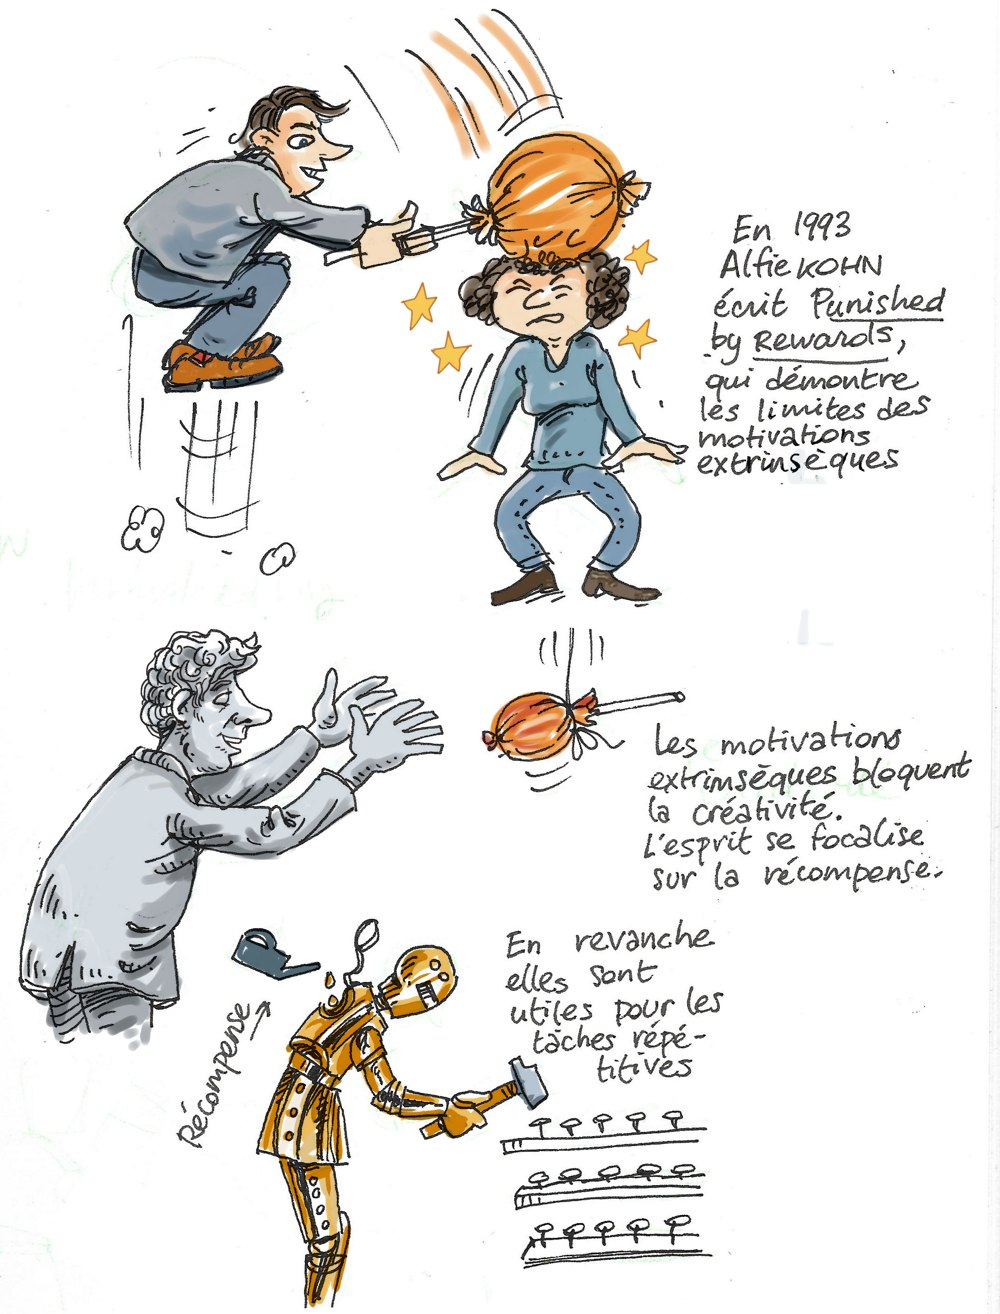
\includegraphics[width=0.92\linewidth]{Figures/Duriez-motiv3.jpg}
        \caption[La punition par la récompense, Kohn~\citeB{kohn1999punished}]{La punition par la récompense, Kohn~\citeB{kohn1999punished}, \textit{ill.} F.~Duriez~\citeURL{motiv_pic}}
        \label{fig:motiv3}
    \end{minipage}
    \hfill
    \begin{minipage}{0.475\linewidth}
        \centering
        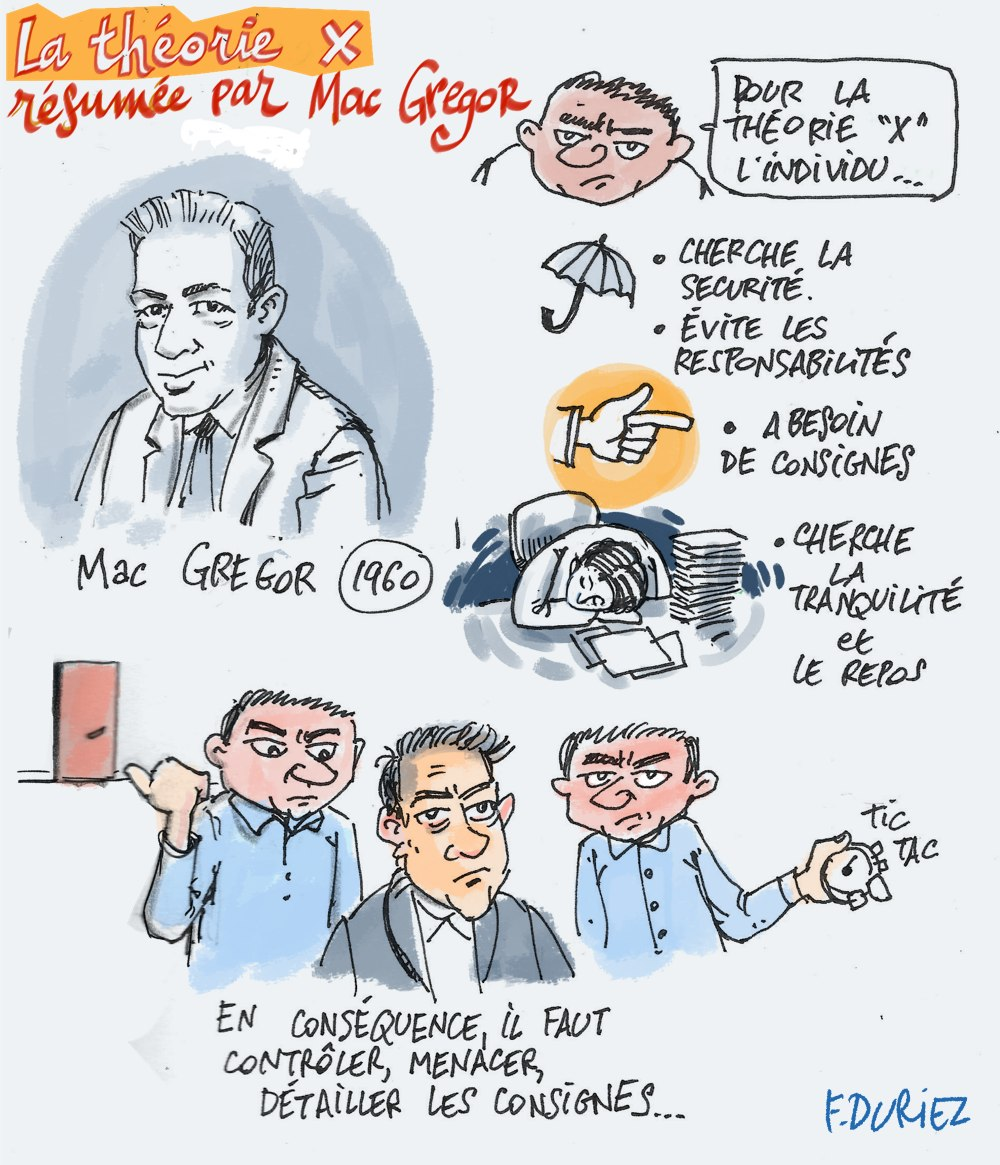
\includegraphics[width=\linewidth]{Figures/Duriez-motiv4.jpg}
        \caption[Théorie X Y, Mac Gregor~\citeB{mcgregor1960theory}]{Théorie X Y, Mac Gregor~\citeB{mcgregor1960theory}, \textit{ill.} F.~Duriez~\citeURL{motiv_pic}}
        \label{fig:motiv4}
    \end{minipage}
    \end{figure}\par%
    En 1957, Mac Gregor~\citeB{mcgregor1960theory} avait opposé 2 théories, la théorie X et la théorie Y. Toutes deux se basent sur un certain nombre de présupposés antagonistes \eg \gui{Naturellement, l'être humain moyen n'aime pas le travail et l'évitera s'il le peut} \textit{vs} \gui{Faire des efforts physiques et mentaux au travail est aussi naturel que s'amuser et se reposer.}
    La 1\iere induira des conséquences comme le besoin pour l'employeur de  guider, contrôler, chronométrer, récompenser ou même menacer l'individu pour le forcer au travail. Tandis que la 2\nde induira des comportements cherchant à expliciter la tâche, à y donner un sens pour l'individu, l'impliquer dans l'organisation, \etc. 
    Le raisonnement total montre comment la 1\iere mène l'individu (et l'organisation) dans un cercle vicieux alors que la 2\nde les mène dans un cercle vertueux.\par%
    Ces résultats deviennent, petit à petit, acquis par une majorité de la population. Cependant, il existe encore de trop nombreux exemples où \cro{la théorie X} est appliquée. Dans l'environnement scolaire, tout bon pédagogue sait \tiret{sans nécessairement pouvoir citer les auteurs ou les expériences} que, plus que des notes ou des compliments, il faut donner du sens aux activités, favoriser les relations, mobiliser plusieurs formes d'intelligences, et varier pour générer de la nouveauté et de la curiosité tout en gardant un \sht{flow} au plus proche de la \sht{ZPD}.
\section{Apports des sciences cognitives}
    \subsection{Les fonctions exécutives}\label{sec:fx-exe}
        Les fonctions exécutives désignent différents processus cognitifs dits de haut niveau. Elles permettent de traiter les informations de manière adaptative en fonction des objectifs et sous-objectifs. Les fonctions exécutives sont nécessaires pour effectuer des activités telles que la planification, l'organisation, l'élaboration de stratégies, pour être attentif et se rappeler les détails, et pour gérer le temps et l'espace~\citeB{chan2008assessment}. Ces fonctions semblent localisées dans le cortex préfrontal~\citeB{wagner2004cognitive}. Mais plusieurs fonctions semblent nécessiter des ressources additionnelles qu'elles trouveront dans d'autres régions du cerveau~\citeB{alvarez2006executive}. Plusieurs modèles de la cognition se basent sur ces fonctions, on peut notamment citer le modèle du système attentionnel superviseur de Donald Norman et Tim Shallice~\citeB{shallice1996domain}. En effet, la hiérarchisation des processus implique l'existence d'un système contrôle, le contrôle exécutif, qui oriente le comportement vers un but~\citeB{taconnat2014fonctions}. La théorie de Miyake, Friedman, Emerson, Witzki, Howerter et Wagner est la théorie dominante dans la littérature sur les fonctions exécutives~\citeB{miyake2000unity}. Ils ont mis en évidence, grâce à une analyse par régression, qu'il existe 3 fonctions spécifiques, qui sont à la fois indépendantes et corrélées entre elles.
    \subsubsection{Trois fonctions principales}    
        \paragraph{La flexibilité mentale (shifting)}
            Il existerait 3 sous-classes correspondant à cette fonction: \Li la flexibilité d'information en mémoire de travail (interne), \ii la flexibilité externe (pour des stimuli environnementaux) et \iii la flexibilité de sources~\citeB{rochat2012difficulties}.
            Celles-ci ont pour point commun de permettre de passer d'une opération cognitive à une autre~\citeB{collette2006exploration}, la capacité à se désengager d'une tâche pour se réengager dans une autre.
            \underline{Évaluation}: 
            \textsc{Le Trail Making Test} (test des tracés)
                    il consiste à faire relier, par le sujet, des chiffres dans l'ordre croissant le plus rapidement possible (1, 2, 3, 4 \etc), puis, il doit recommencer mais en alternant des chiffres et des lettres (1-A, 2-B, 3-C, \etc).
                \textsc{Le Plus-Minus Test}
                    , ici, dans un premier temps, le sujet est entraîné à faire une série d'additions sur des nombres à deux chiffres, puis il est entraîné à faire une série de soustractions, et enfin, il doit alterner les additions et les soustractions. 
                Le \gui{coût de shifting} est calculé en faisant la différence entre la 2\nd et la 1\iere tâche. Reitan 1958~\citeB{reitan1958validity}.
                \textsc{Le Wisconsin Card Sorting Test}
                    est un test neuropsychologique élaboré par David A. Grant et Esta A. Berg en 1948~\citeB{grant1948behavioral}. On présente au sujet quatre cartes composées d'items qui diffèrent de par leur couleur, leur forme et leur nombre. La personne a, dans sa main, le paquet du reste des cartes. Sa tâche est de catégoriser une à une les cartes restantes en les posant sur l'un des quatre tas. On ne lui donne pas de critère pour organiser ses cartes mais l'examinateur lui signifie (uniquement par oui ou par non) si le critère choisi est le bon. Le sujet organise alors ses cartes selon le premier critère choisi pendant quelques cartes, puis à un moment, l'examinateur décide de changer de critère et le sujet doit retrouver le nouveau critère de classification.
                    On mesure ici les erreurs de persévérance (\cad quand le sujet persévère dans le critère qui lui est devenu routinier). Cela permet de déterminer la capacité du sujet à intégrer le feedback externe, mais également s'il est capable d'inhiber une réponse qui lui est devenue routinière.
        \paragraph{La mise à jour (updating)}
            La mémoire de travail étant limitée, cette fonction permet de maintenir à jour les items en fonction de leur pertinence: elle remplace l'information qui n'est plus pertinente avec l'information plus récente et plus pertinente~\citeB{morris1990memory}. Cela signifie que son contenu est modifié sur la base de l'information entrante plus récente~\citeB{shimamura2000role} en fonction d'un but et que cette mise à jour nécessite la surveillance et le codage de l'information.
            \underline{Évaluation}:
            \textsc{Le N-Back Test}
                est une tâche de reconnaissance, Smith et Jonides 1997~\citeB{smith1998neuroimaging}, Les sujets sont invités à indiquer si un élément dans une liste correspond à l'élément qui a été présenté n positions avant. Exemple, pour n=2, dans la liste \cro{F-B-L-B} il y a un \textit{match 2-back} (B-B), tandis que dans la liste \cro{F-B-L-G} on parle de \textit{décalage 2-back}. Le nombre et la qualité des leurres~\citeB{szmalec2011control} influent sur la capacité du sujet à exécuter la tâche rapidement et sans erreur.
        \paragraph{L'inhibition}
            C'est une fonction capitale du système cognitif. Elle correspond à un ensemble de mécanismes permettant la suppression ou la rétention de processus ou d'actions qui perturberaient le bon achèvement de l'objectif en cours~\citeB{dempster1992rise}. Elle permet également d'occulter des éléments non pertinents~\citeB{bjorklund1995evolution}. C'est une fonction présente dans l'ensemble de nos interactions avec l'environnement~\citeB{burke1991improving} y compris dans des compétences sociales et la régulation émotionnelle~\citeB{urben2011inhibition}.
            \underline{Évaluation}
                \textsc{La tâche Stroop}
                    \citeB{stroop1935studies} est un tâche où il est demandé au sujet d'énoncer, à voix haute, la couleur de l'encre des mots d'une liste, exemple: \textcolor{red}{bleu}, \textcolor{blue}{rouge}, \textcolor{red}{bleu}, \textcolor{green}{jaune}, \textcolor{yellow}{vert}, \textcolor{blue}{rouge}, \textcolor{yellow}{vert}, \textcolor{green}{jaune}, \textcolor{blue}{rouge}, \textcolor{blue}{vert}, \textcolor{green}{bleu}, \textcolor{green}{jaune}, \textcolor{yellow}{rouge}, \textcolor{blue}{jaune}, \textcolor{yellow}{vert}, \textcolor{green}{jaune}, \textcolor{blue}{rouge}. Les gens ont une tendance à lire automatiquement le mot et cela conduit à des interférences entre le mot de couleur et la couleur de l'encre. Pour réussir la tâche, il est important d'inhiber la tendance à lire les mots. Le nombre d'erreurs détermine la mesure de la capacité d'inhibition du sujet.
                \textsc{La tâche Flanker}
                    est une tâche de réaction qui est conçue pour mesurer la capacité de pointer l'attention visuelle, en inhibant les informations gênantes. Dans cette tâche, les participants doivent donner une réponse rapide de gauche ou de droite à une flèche centrale, tout en ignorant les flèches d'accompagnement congruentes (par exemple, < < < < <) ou non congruentes (par exemple, < < > < <). Les gens ont une tendance à traiter automatiquement les informations de distraction, car ils sont généralement plus lents sur les stimuli non congruents que sur les stimuli congruents. Eriksen et Eriksen 1974~\citeB{eriksen1974effects}.
    \subsection{La théorie de la charge cognitive}\label{sec:cog_load}
        La charge cognitive est introduite par le psychologue John Sweller dans les années 80~\citeB{sweller1988cognitive}. Elle concerne la quantité d'informations que la mémoire de travail peut contenir à la fois. La mémoire de travail étant limitée~\citeB{miller1956magical}, les expériences d'apprentissage doivent être conçues de manière à réduire la charge de la mémoire de travail afin de promouvoir l'acquisition de schéma.
        \subsubsection{Deux types d’apprentissages}
            Connaissances primaires et secondaires soumises à des contraintes différentes:
            \paragraph{Primaires}
                Ce sont des apprentissages implicites comme par exemple, apprendre sa langue maternelle, reconnaître les visages, les émotions, \etc, c'est une adaptation à l’environnement social et physique de l'individu. Il y a pas (ou peu) d’efforts attentionnels, ce sont des apprentissages qui s'effectuent relativement rapidement et sans en avoir conscience. L'immersion, l’exploration, les jeux et les relations sociales favorisent leur développement. La généralisation et le transfère de compétences pour les tâches relevant de ce type d'apprentissage est facile et fréquent.
            \paragraph{Secondaires}
                Ce sont des apprentissages explicites: on apprend consciemment, avec un effort, c’est parfois long et difficile. Ce sont des apprentissages utiles pour la préparation à la vie future (sociale, travail, langage écrit, maths par exemple) et l'élaboration de schémas complexes. Une pratique intense, sur la durée, et enseignée est nécessaire à ce type d'apprentissage conscient et délibéré. La motivation extrinsèque (portée par autrui) est parfois nécessaire et souvent utile. Le processus de généralisation est difficile et pénible, voir assez vain pour enseigner des connaissances générales.
            %Si on fait rentrer des principes des connaissances primaires (immersion, relations sociales, jeux \etc) pour apprendre des connaissances secondaires en classe, ça se passe mieux. Mais il faut que le but soit l’apprentissage explicite, que ça reste une tâche consciente, que se soit que la méthode qui soit améliorée.
            %Comment prendre en compte tout ça quand on conçoit un support pédagogique ?
            Quand un humain apprend une connaissance secondaire, il doit fournir un effort mental. Cet effort est proportionnel à la charge induite par la tâche. Il y a 3 types de charges:
            \begin{enumerate}\myItemStyle
                \item Charge essentielle, c'est ce qui doit être appris, les connaissances réelles qui doivent être acquises (apprentissage du théorème de Pythagore par exemple). Effort pour construire la connaissance.
                \item Charge intrinsèque, c'est l'effort réalisé pour mettre en œuvre la tâche que propose l'enseignant. Par exemple, un problème de mathématiques: il a pour objet de  mettre en œuvre la connaissance. Mais si cette tâche pratique est trop dure, il n’y aura plus de ressources disponibles pour construire de la nouvelle connaissance. Le moyen (la tâche, \eg le problème de mathématiques) peut parfois devenir un frein au but (l’apprentissage, \eg le théorème de Pythagore).
                \item Charge extrinsèque, c'est toutes les informations superflues ce qui ne sont pas strictement utiles à l’apprentissage mais qui sont présentes dans le contexte et qui biaisent ou distraient l'individu. Par exemple, les bugs, les erreurs de design, les bavardages, \etc.
            \end{enumerate}
        \subsubsection{Différents effets}\label{sec:effect}
            \paragraph{L’effet de non spécification du but}
                Il peut parfois être bien de ne pas préciser immédiatement le but. Par exemple, dans la consigne \cro{trouvez la valeur de l’angle BDE}, l’élève doit trouver par lui même les buts et calculs intermédiaires. 
                Alors que si la consigne est \cro{trouver un maximum d’angles possibles}, il se rend compte qu’il y a des étapes intermédiaires nécessaires pour trouver certains angles, et il ne se sent pas bloqué.
                Dans un second temps, en leur donnant la consigne \cro{trouvez  la valeur de l’angle BDE}, ceux du 2\nd groupe, n'ayant jamais eu cette consigne, obtiennent de meilleurs résultats~\citeB{sweller1988cognitive}.%e la condition 2 ont appris qu’il fallait trouver un angle à partir d’autres et ils y arriveront mieux.
            \paragraph{L’effet du problème résolu}
                Il peut parfois être plus pertinent de demander à des élèves d’étudier un problème résolu, une procédure écrite, plutôt que de leur faire résoudre directement le problème ou créer la procédure de résolution~\citeB{anderson1990cognitive}. Cela permet de baisser l’exigence attentionnelle. Et donc, fournir le résultat et la procédure puis les retirer au fur et à mesure de la progression de l'élève permet de ne pas surcharger l'apprentissage en le décomposant.
            \paragraph{L’effet d’attention partagée}
                Lorsque l’objectif le permet, il faut essayer de diminuer la charge due au design de l’information. Si l’information pertinente est placée dans un endroit pertinent, cela enlève de la charge cognitive car l’élève n’a pas à superposer mentalement les informations~\citeS{sec:affordance}. Si 2 informations sont nécessaires, il faut arriver à les mettre en relation (sémantiquement, visuellement, géographiquement, \etc) pour ne pas augmenter la charge due à l’éloignement. Éviter l’attention partagée et l’effort mental superflu~\citeS{sec:double-tache}.
            \paragraph{L’effet de modalité et de redondance}
                Utiliser des modalités sensorielles différentes et adaptées à la tâche mise en œuvre et aux connaissances engagées est primordial: apprendre une poésie (qu'il faudra réciter) uniquement par de la lecture silencieuse n'est pas efficace.
                Mais, multiplier les modalités sensorielles pour une seule tâche n'est pas bénéfique: l'une ou l'autre va détériorer l’apprentissage en le surchargeant~\citeB{penney1989modality} (exemple: lire et entendre le même texte simultanément).
            %Attention: Tout ceci est valable dans le domaine de l’apprentissage complexe uniquement. \paragraph{Effet d’isolement des éléments interactifs}
                Si l’apprentissage implique de comprendre de nombreux éléments en interaction, il est parfois plus efficace de présenter, d’abord les éléments de manière isolée, puis dans un second temps, de présenter leurs interactions duales, puis de les généraliser dans l’ensemble total~\citeB{ayres2013can}. Cependant dans certains cas, les éléments n'ont pas nécessairement de sens ou de pertinence, pris isolément, dans ce cas, il est nécessaire de passer par une phase préliminaire de présentation de la structure complète avant de pouvoir en isoler les éléments afin de les expliciter progressivement.
            \paragraph{D'autres effets}
                Guider, au début, puis enlever petit à petit le guidage; montrer plusieurs problèmes similaires; multiplier les exemples; faire imaginer préalablement à l'élève la réalisation de la procédure qu'il aura à exécuter; effectuer des exercices d'évaluation; sont autant d'éléments qui améliorent les apprentissages~\citeB{sweller1988cognitive}. Cependant, une fois un niveau d'expertise suffisant, on observe un effet de reversement concernant les effets précédemment cités qui deviennent alors délétères à l'apprentissage~\citeB{sweller2003expertise}. Une stratégie semblant rester efficace, est, l'objectif d'auto-explication~\citeB{chebbihi2018autoexp}: devoir s’expliquer quelque chose à soi même est souvent plus efficace que simplement essayer de faire ou de comprendre. Une consigne \cro{lis ce texte, et essayes de te l’expliquer} est plus efficace qu'une consigne: \cro{lis ce texte, et essayes de le comprendre}.
                Enfin, nous pouvons signaler qu'un travail collectif n'est bénéfique que dans le cadre d'une tâche qui ne peut pas être réalisée seule.